\documentclass{article}
\usepackage[utf8]{inputenc}
\usepackage{url}
\usepackage{graphicx}
\graphicspath{ {./} }


\title{Automatisation du prétraitement de photographies de portraits de mandrills}
\author{Maxime Boucher}
\date{Compte rendu 5}

\begin{document}

\maketitle

Depuis la dernière fois, le jeu de données s'est agrandi de près de  10000 images (environ 20000 vers environ 30000 images).
Cela a nécessairement rendu les résultats passés "périmés".\\

On a donc un nouveau jeu de données auquel on peut appliqué notre modèle, que ce soit pour 0FaceView (détermination face/profil) et 1FaceQual (détermination qualité). \\

Le meilleur CNN (basé sur EfficientNet) a perdu beaucoup en efficacité notamment sur les classes 1FaceQual0 et 1FaceQual1 par rapport à la dernière fois. Les erreurs sont largement dans présentes dans la cellule d'à coté, donc cela signifie que le réseau a plus de mal à discerner des classes distinctes. Diverses raisons sont possibles : sous apprentissage, sur apprentissage, bruit dans le dataset. 
\begin{center}
    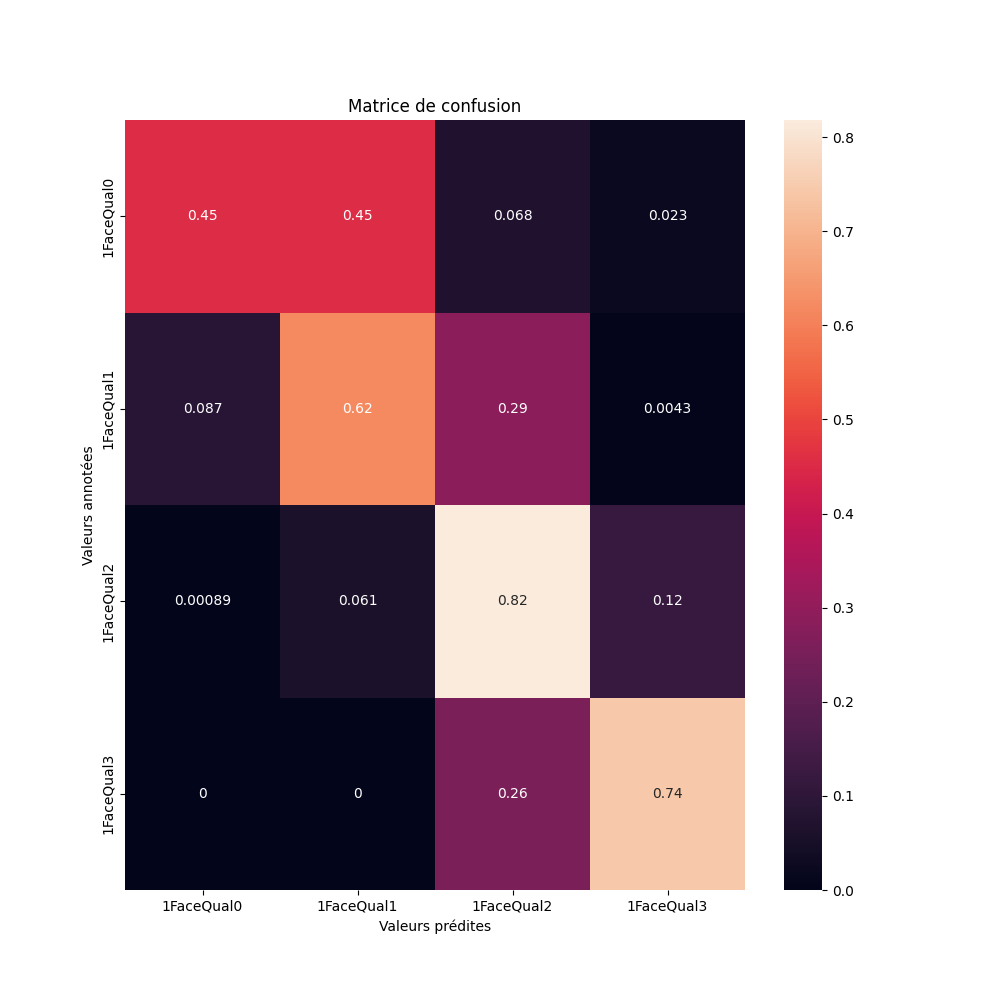
\includegraphics[width=200]{imgs/qualité/cr5/confusion_fine.png}
\end{center}

Concernant face/profil, le meilleur résultat provient a priori d'un entraînement sur VGG 16.
\begin{center}
    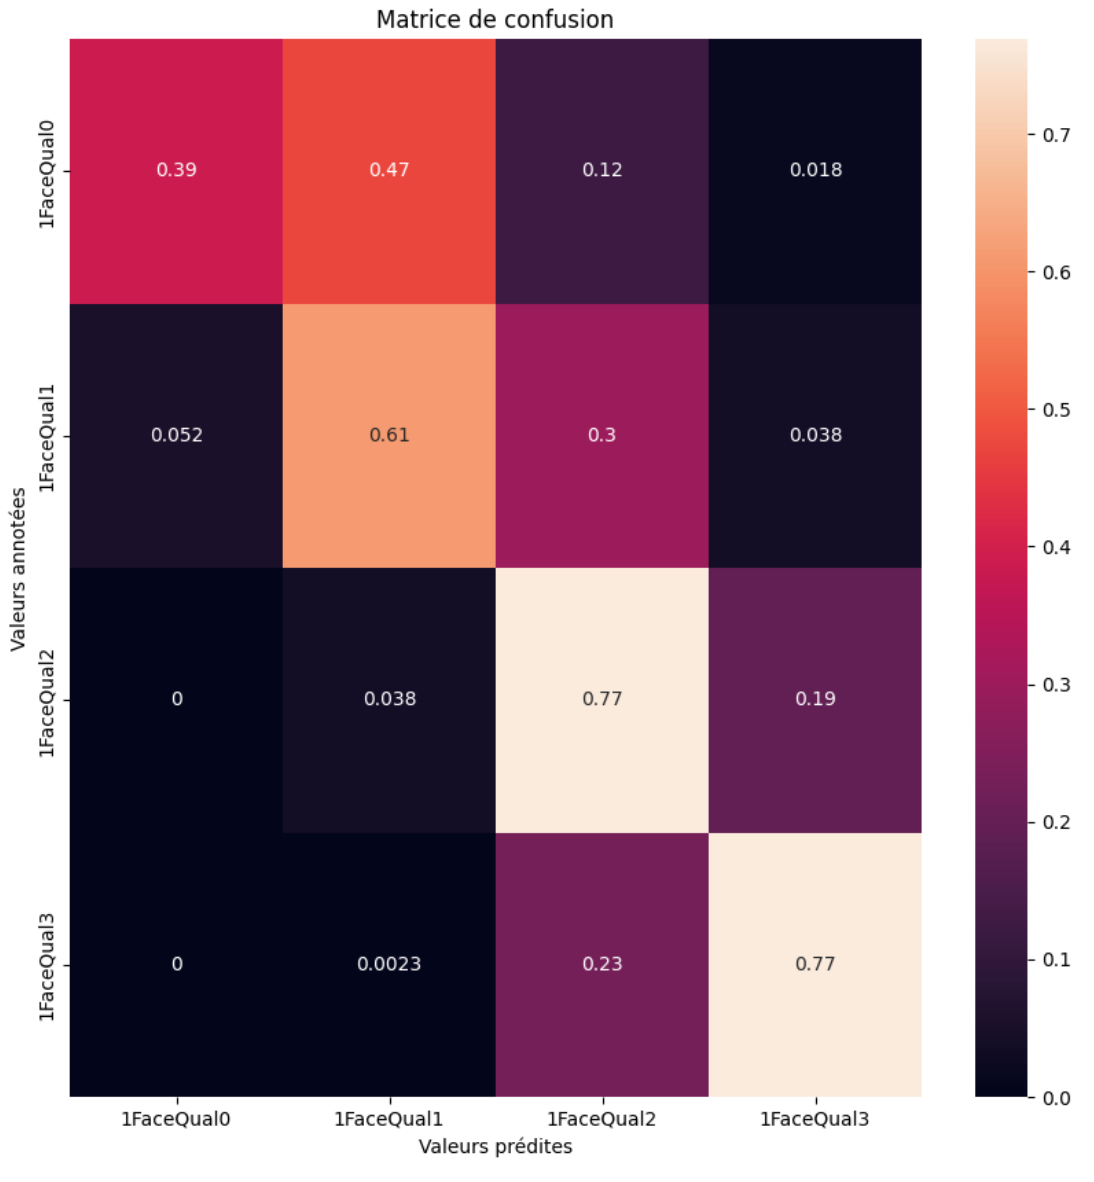
\includegraphics[width=200]{imgs/qualité/cr5/confusion.png}
\end{center}

90 pourcents des échantillons, que ce soit dans la classe 0FaceView0 (profil) ou 0FaceView1 (face), sont correctement prédis. \\

cleanlab est un package potentiellement intéressant dans le cadre de datasets avec du bruit. Je vais explorer cette piste en plus d'affiner des paramètres du CNN.
https://github.com/cgnorthcutt/cleanlab/

\end{document}
